\documentclass[professionalfonts,compress,unicode,aspectratio=169]{beamer}
\usetheme{Moscow}

\usepackage[utf8]{inputenc}
\usepackage[T2A]{fontenc}
\usepackage[main=russian,english]{babel}

\usepackage{amsmath,amssymb}

\renewcommand{\thefootnote}{\fnsymbol{footnote}}
\hypersetup{pdfauthor={Ivan Tsybulin}}


\graphicspath{{images//}}

\title[Методы Рунге-Кутты]{Задача Коши. Методы Рунге-Кутты. Жесткие задачи}
\author[Цыбулин И.В.]{Скалько Юрий Иванович\\
\textbf{Цыбулин Иван}}
\date{}

\newcommand{\colorhref}[2]{\href{#1}{\textcolor{miptbase!30!black}{#2}}}

\begin{document}

\begin{frame}[plain]
\titlepage
\end{frame}

\def\L{\mathcal{L}}
\renewcommand{\vec}[1]{\boldsymbol{\mathbf{#1}}}

\section{Обыкновенные дифференциальные уравнения}
\begin{frame}\frametitle{Задача Коши}
	Дано обыкновенное дифференциальное уравнение 1го порядка и начальное условие
	\begin{align*}
	\frac{d\vec y(t)}{dt} &= \vec G(t, \vec y(t))\\
	\vec y(0) &= \vec y_0
	\end{align*}
	Требуется найти решение $\vec y(t)$ при $t \in [0, T]$
\end{frame}

\section{Методы Рунге-Кутты}
\subsection{Общие положения}
\begin{frame}\frametitle{Методы Рунге-Кутты}
	Методы Рунге-Кутты относятся к \emph{одношаговым методам}, то есть они позволяют по
	значению решения $\vec u_{n}$ вычислить значение в следующей точке $\vec u_{n+1}$.

	Каждый шаг метода состоит из нескольких \emph{стадий}, на которых вычисляются вспомогательные
	наклоны $\vec k$. Вычисление наклонов в специально подобранных промежуточных точках позволяет
	получить метод с высоким порядком аппроксимации.
\end{frame}

\begin{frame}\frametitle{Общая схема методов Рунге-Кутты}
	Каждый метод Рунге-Кутты характеризуется набором коэффициентов $a_{ij}, b_j, c_i$.
	Один шаг метода проводится по следующей схеме:
	\begin{columns}[T]
	\begin{column}{.5\textwidth}
	\begin{align*}
	\vec k_1 = \vec G(t_n + c_1 \tau&, \vec u_n + \tau\sum_{j=1}^s a_{1j} \vec k_j)\\
	&\vdots\\
	\vec k_s = \vec G(t_n + c_s \tau&, \vec u_n + \tau\sum_{j=1}^s a_{sj} \vec k_j)\\
	\frac{\vec u_{n+1} - \vec u_n}{\tau} &= \sum_{j=1}^s b_j \vec k_j
	\end{align*}
	\end{column}
	\begin{column}{.5\textwidth}
	\begin{figure}%
	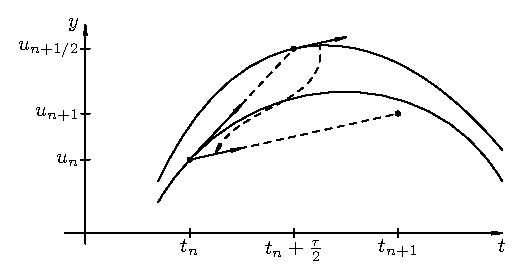
\includegraphics[width=.7\columnwidth]{rk-0.eps}%
	\begin{align*}
	\vec k_1 &= \vec G(t_n, \vec u_n)\\
	\vec k_2 &= \vec G\left(t_n + \frac{\tau}{2}, \vec u_n + \frac{\tau}{2} \vec k_1\right)\\
	&\frac{\vec u_{n+1} - \vec u_n}{\tau} = \vec k_2
	\end{align*}
	\end{figure}
	\end{column}
	\end{columns}
\end{frame}

\begin{frame}\frametitle{Решения, полученные методами Рунге-Кутты}
	Ниже показаны решения задачи о движении тела в поле тяжести, рассчитанные
	различными методами Рунге-Кутты с автоматическим выбором длины шага по
	времени для обеспечения точности $\varepsilon = 10^{-3}$

	\begin{figure}
	\centering
	\includegraphics<1>[width=.5\textwidth]{Traj1.pdf}%
	\includegraphics<2>[width=.5\textwidth]{Traj2.pdf}%
	\includegraphics<3>[width=.5\textwidth]{Traj4.pdf}%
	\only<1>{\caption{Метод Эйлера, $1260$ шагов}}%
	\only<2>{\caption{Явный метод центральной точки, $190(\sim 380)$ шагов}}%
	\only<3>{\caption{Метод Рунге-Кутты 4-го порядка, $66(\sim 264)$ шагов}}%
	\end{figure}
\end{frame}

\begin{frame}\frametitle{Таблица Бутчера}
	Коэффициенты $a_{ij}, b_j, c_i$ удобно представлять в виде \emph{таблицы Бутчера}
	\begin{equation*}
	\begin{array}{c|cccccc}
	c_1 & a_{11} & a_{12} & \dots & a_{1s}\\
	c_2 & a_{21} & a_{22} & \dots & a_{2s}\\
	\vdots & & & \ddots & \\
	c_s & a_{s1} & a_{s2} & \dots & a_{ss}\\
	\hline
	& b_1 & b_2 & \dots & b_s
	\end{array}
	\end{equation*}
	\pause
	Например, явному методу средней точки соответствует таблица
	\begin{equation*}
	\begin{array}{c|cccccc}
	0 & 0 & 0\\
	\frac{1}{2} & \frac{1}{2} & 0\\
	\hline
	& 0 & 1
	\end{array}
	\end{equation*}
\end{frame}

\begin{frame}\frametitle{Явные, полуявные и неявные методы Рунге-Кутты}
	В зависимости от коэффициентов $a_{ij}$ вычисления наклонов $\vec k_i$ могут
	происходить по-разному.

	\begin{itemize}
	\item
	Если матрица $a_{ij}$ имеет ненулевые элементы ниже главной диагонали ($a_{ij} = 0, i\geq j$),
	то метод называется \emph{явным}. При этом все наклоны $\vec k_i$ вычисляются через предыдущие без необходимости
	решать уравнения.

	\item
	Если матрица $a_{ij}$ имеет ненулевые элементы и на главной диагонали ($a_{ij} = 0, i > j$),
	то метод называется \emph{полуявным}. При этом все наклоны $\vec k_i$ вычисляются последовательно из уравнений.

	\item
	Иначе, метод называется \emph{неявным}, и необходимо решать систему
уравнений для всех $\vec k_i$ одновременно.
	\end{itemize}
\end{frame}

\subsection{Аппроксимация}
\begin{frame}\frametitle{Разложение наклонов}
	Поскольку метод Рунге-Кутты определяется своими коэффициентами, можно сформулировать условия на коэффициенты метода, при котором
	он имеет определенный порядок аппроксимации. Найдем условия первого и
второго порядков, для этого подставим $\vec u_n = [\vec y]_n$, где $\vec y(t)$ ---
	решение задачи Коши:
	\begin{align*}
	\vec k_i &= \vec G(t_n + c_i \tau, [\vec y]_n + \tau \sum\nolimits_{j=1}^s a_{ij}
\vec k_j) =\\
			&= [\vec G]_n + \tau c_i [\vec G_t]_n + \tau \sum\nolimits_{j=1}^s
a_{ij} [\vec G_y]_n \vec k_j + O(\tau^2) = \\
			&= [\vec G]_n + \tau c_i [\vec G_t]_n + \tau \sum\nolimits_{j=1}^s
a_{ij} [\vec G_y]_n \Big([\vec G]_n + O(\tau)\Big) + O(\tau^2) = \\
			&= [\vec G]_n + \tau c_i [\vec G_t]_n + \tau \sum\nolimits_{j=1}^s
a_{ij} [\vec G_y]_n [\vec G]_n + O(\tau^2)
	\end{align*}
\end{frame}

\begin{frame}\frametitle{Условия первого и второго порядка}
	Выразим производные $\vec y'$ и $\vec y''$ из уравнения:
	$
		[\vec y']_n = [\vec G]_n, \qquad [\vec y''] = [\vec G_t + \vec G_y \vec G]_n
	$
	\begin{align*}
	\vec k_i &= [\vec G]_n + \tau c_i [\vec G_t]_n + \tau \sum_{j=1}^s a_{ij}
[\vec G_y]_n [\vec G]_n + O(\tau^2)\\
	\sum_{j=1}^s b_j k_j &=
	\sum_{j=1}^s b_j [\vec G]_n + \tau \sum_{j=1}^s b_j c_j [\vec G_t]_n + \tau
\sum_{i,j=1}^s b_i a_{ij} [\vec G_y]_n[\vec G]_n \\
	\frac{[\vec y]_{n+1}-[\vec y]_n}{\tau} &= [\vec G]_n + \frac{\tau}{2}[\vec
G_t]_n + \frac{\tau}{2}[\vec G_y]_n [\vec G]_n + O(\tau^2)
	\end{align*}
	\pause
	Условие $1$-го порядка аппроксимации: $\displaystyle \sum_{j=1}^s b_j = 1$.

	Условия $2$-го порядка аппроксимации: $\displaystyle \sum_{j=1}^s b_j c_j = \sum_{i,j=1}^s b_i a_{ij} = \frac{1}{2}$.
\end{frame}

\begin{frame}\frametitle{Барьеры Бутчера}
	Бутчер доказал несколько теорем о связи порядка аппроксимации и количества стадий у методов Рунге-Кутты.
	Явные методы с $s<5$ стадиями могут иметь порядок не выше $s$, но после $s=5$ стадий наступает, так называемый,
	\emph{первый барьер Бутчера}, и порядок аппроксимации не превышает $s-1$. При увеличении $s$ возникают все новые барьеры, понижающие
	порядок аппроксимации.

	Однако, для неявных методов ограничение не такое строгое. Например есть семейство методов (Гаусса), у которых порядок аппроксимации $2s$ при любом числе стадий.
\end{frame}

\subsection{Устойчивость}
\begin{frame}\frametitle{Устойчивость}
	Если правая часть ОДУ $G(t,y)$ липшицева по $y$ с константой $L$
	$$\|\vec G(t,\vec y) - \vec G(t,\vec v)\| \leq L \|\vec y-\vec v\|,$$
	то несложно показать, что константа устойчивости для методов Рунге-Кутты порядка
	$C \sim \exp\{O(L)T\}$. Следовательно, имеет место сходимость решения разностной задачи к решению дифференциальной задачи.

	Но в случаях, когда $LT \gg 1$ константа устойчивости становится огромной.
	Вспомним, что ошибка сходимости связана с ошибкой аппроксимации
	соотношением
	$$\varepsilon_\text{сх} = C	\varepsilon_\text{аппр}(\tau).$$
	Для того, чтобы обеспечить малую ошибку сходимости необходимо выбирать очень
	маленький шаг по времени $\tau$.
\end{frame}

\section{Жесткие задачи Коши}
\subsection{Жесткость}
\begin{frame}\frametitle{Жесткие задачи}
	Жесткие системы ОДУ описывают, как правило, одновременно проходящие очень быстрые и очень медленные процессы. 
	Например, в задачах химической кинетики бывают различия в скоростях реакций до $10^{15}$ раз.
	\pause
	Оказывается, что быстро протекающие процессы, даже быстро закончившись, продолжают влиять на численное решение задачи, 
	вынуждая рассчитывать решение с очень малым шагом по времени, где это, казалось бы, совершенно не требуется (решение довольно гладкое).
\end{frame}

\subsection{Пример жесткой задачи}
\begin{frame}\frametitle{Поле решений жесткой задачи}
	\begin{columns}[T]
	\begin{column}{.5\textwidth}
	\vspace{1in}
	Поле решений уравнения
	\begin{align*}
	\dot x &= -0.5 x + 20 y\\
	\dot y &= -20 y
	\end{align*}
	содержит резкие повороты --- индикатор жесткости задачи.
	\vspace{1in}
	\end{column}
	\begin{column}{.5\textwidth}
	\begin{figure}%
	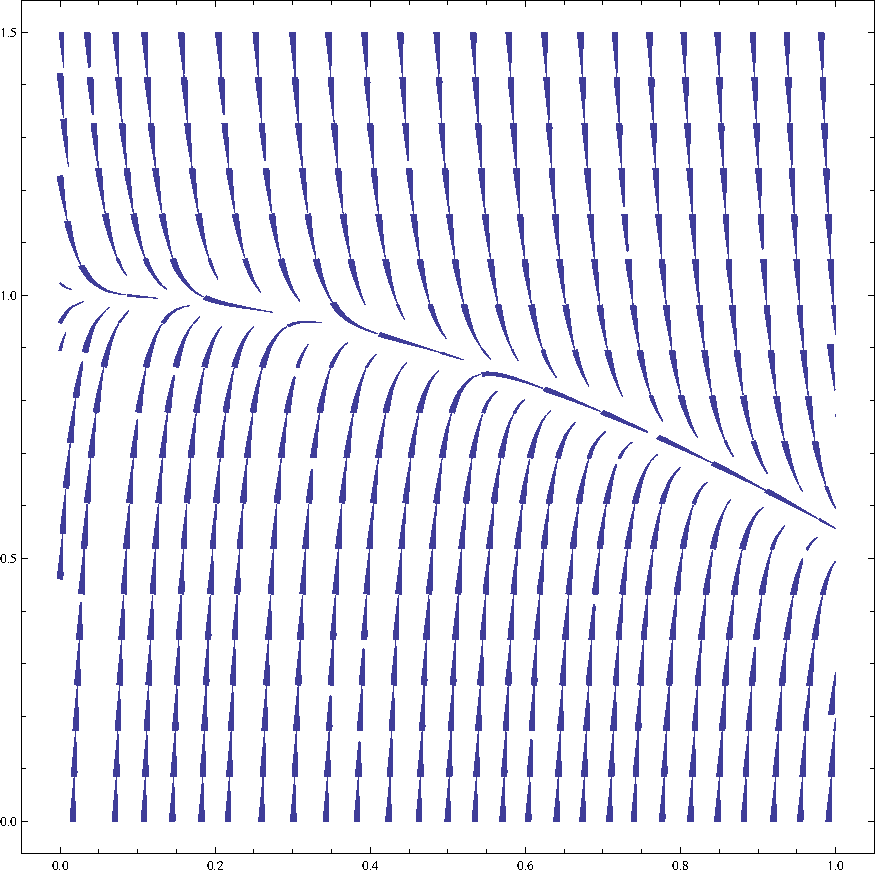
\includegraphics[height=.75\textheight]{stiff.pdf}%
	\end{figure}
	\end{column}
	\end{columns}
\end{frame}

\subsection{Определение жесткой задачи}
\begin{frame}\frametitle{Определение жесткой задачи}
	Можно дать следующее определение:

	Жесткая задача --- это такая задача, у которой собственные числа матрицы Якоби $G_y$
	разбиваются на две части --- мягкую часть спектра $|\lambda_i| < \ell$ и
жесткую часть спектра $\operatorname{Re} \Lambda_i < -L$, причем $\ell \ll L$.
Величина $L/\ell$ называется показателем жесткости.
	\begin{figure}%
	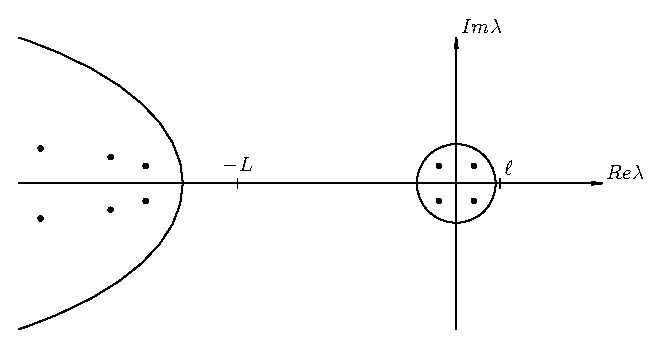
\includegraphics[height=.6\textheight]{sp.eps}%
	\caption{}%
	\label{}%
	\end{figure}
\end{frame}

\subsection{Жесткая устойчивость}
\begin{frame}\frametitle{Модельное уравнение}
	Выяснить, как на жестких задачах себя ведет тот или иной метод, можно на модельном уравнении
	\[
	y' = \lambda y,\quad \operatorname{Re} \lambda < 0
	\]
	Все линейные численные методы для решения этого уравнения будут иметь вид
	\[
	u_{n+1} = r(\lambda \tau) u_n,
	\]
	где $r(z)$ --- функция, зависящая только от метода. Эта функция называется
\emph{функцией устойчивости метода}.
	Если при данном сочетании $\lambda$ и $\tau$ значение функции $r(\lambda \tau)$ по модулю больше единицы, решение будет экспоненциально возрастать, что
	противоречит реальному поведению решения при $\operatorname{Re} \lambda < 0$.
	Область комплексной плоскости $\mathbb{C}$, в которой $|r(z)| < 1$
называется \emph{областью устойчивости метода}.
\end{frame}

\begin{frame}\frametitle{Функция и область устойчивости}
	Если при данном $\tau$ вся жесткая часть спектра попадает в область устойчивости, она гарантированно не будет экспоненциально возрастать, и
	решать систему ОДУ можно только обращая внимание на мягкую часть спектра.

	\begin{columns}[T]
	\begin{column}{.5\textwidth}
	Для явного метода Эйлера
	\[
	\frac{u_{n+1}-u_n}{\tau} = \lambda u_n
	\]
	функция устойчивости
	\begin{align*}
	u_{n+1} &= (1 + \tau \lambda)u_n = (1+z) u_n\\
	r(z) &= 1+z
	\end{align*}
	\end{column}
	\begin{column}{.5\textwidth}
	\begin{figure}%
	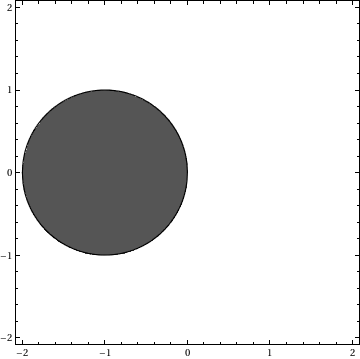
\includegraphics[height=.55\textheight]{euler.png}%
	\end{figure}
	\end{column}
	\end{columns}
\end{frame}

\begin{frame}\frametitle{Область устойчивости}
	\begin{columns}[T]
	\begin{column}{.5\textwidth}
	Для неявного метода Эйлера
	\[
	\frac{u_{n+1}-u_n}{\tau} = \lambda u_{n+1}
	\]
	функция устойчивости
	\begin{align*}
	u_{n+1} &= \frac{u_n}{1 - \tau \lambda} = \frac{u_n}{1 - z}\\
	r(z) &= \frac{1}{1-z}
	\end{align*}
	\end{column}
	\begin{column}{.5\textwidth}
	\begin{figure}%
	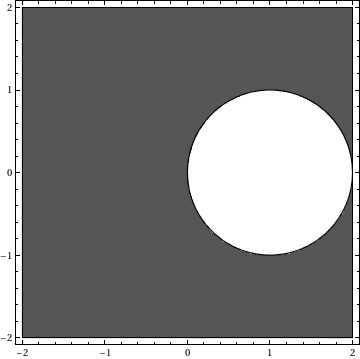
\includegraphics[height=.75\textheight]{euleri.png}%
	\end{figure}
	\end{column}
	\end{columns}
\end{frame}

\begin{frame}\frametitle{Допустимый шаг $\tau$ для жесткой задачи}
	Если шаг по времени $\tau$ таков, что все собственные числа $\Lambda_i$
задачи из жесткой части спектра попадают в область устойчивости данного метода
	\[
		|r(\tau \Lambda_i)| \leq 1,
	\]
	то с таким шагом решать жесткую задачу можно.

	Если это требование нарушить,
жесткие компоненты решения начнут экспоненциально возрастать (хотя обязаны
стремится к нулю!).
	\begin{figure}
	\centering
	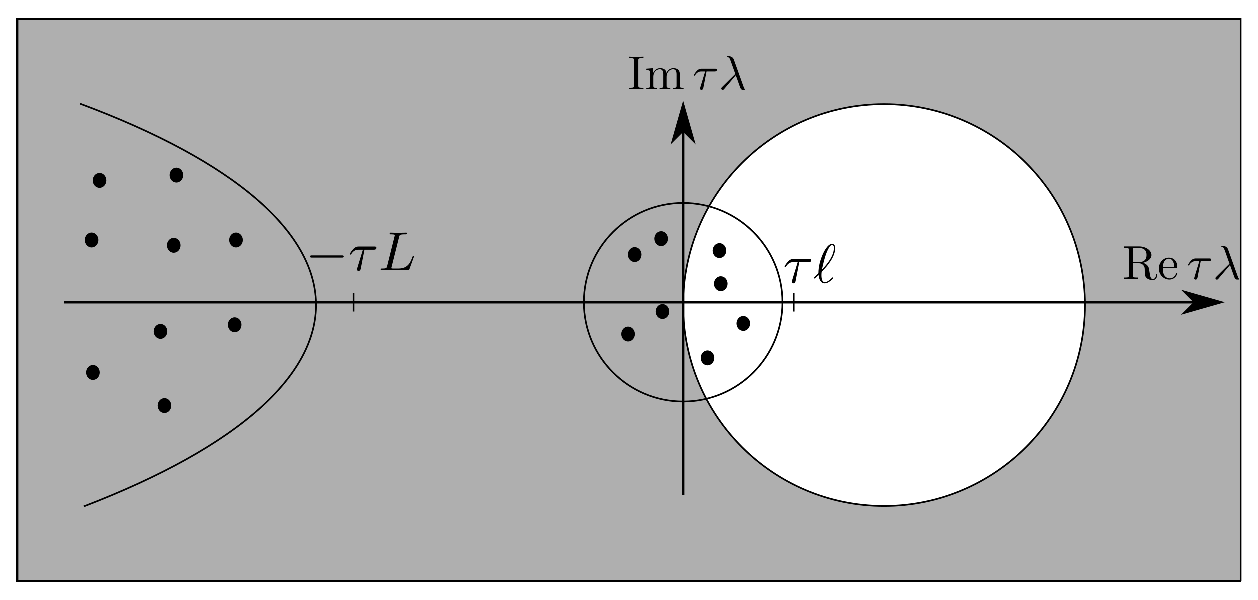
\includegraphics[height=.4\textheight]{stabreg.eps}
	\end{figure}
\end{frame}

\begin{frame}\frametitle[A- и L- устойчивость]{$A$- и $L$-устойчивость}
	По виду области устойчивости методы можно дополнительно классифицировать. Это позволяет выбирать метод,
	наиболее подходящий для конкретного вида жесткой части спектра задачи.

	\begin{itemize}
		\item $A$-устойчивость означает, что во всей полуплоскости $\operatorname{Re} z < 0$ метод устойчив, т.е. $|r(z)| < 1$.
			Такой меотд годится для любых жестких задач.
		\item $A(\alpha)$-устойчивость означает, что в конусе $|\operatorname{Im} z| < -\tg \alpha \operatorname{Re} z$ метод устойчив. $A$-устойчивость 
		эквивалентна $A(90^\circ)$.
			Такой метод годится для задач, у который жесткий спектр прижат к
действительной оси. Чем больше $\alpha$, тем универсальнее метод.
		\item $L$-устойчивость означает, что $\lim_{z \rightarrow -\infty} r(z) = 0$. Это свойство говорит, что при большом шаге $\tau$ жесткая часть спектра 
		стремится к нулю достаточно быстро.
			Эти методы хороши тем, что допускают интегрирование погранслоя с
большим шагом. Не L-устойчивые методы осциллируют при выходе из погранслоя.
	\end{itemize}
\end{frame}

\begin{frame}\frametitle[A- и L- устойчивые методы]{$A$- и $L$-устойчивые методы}
	\begin{figure}
	\centering
	\only<1>{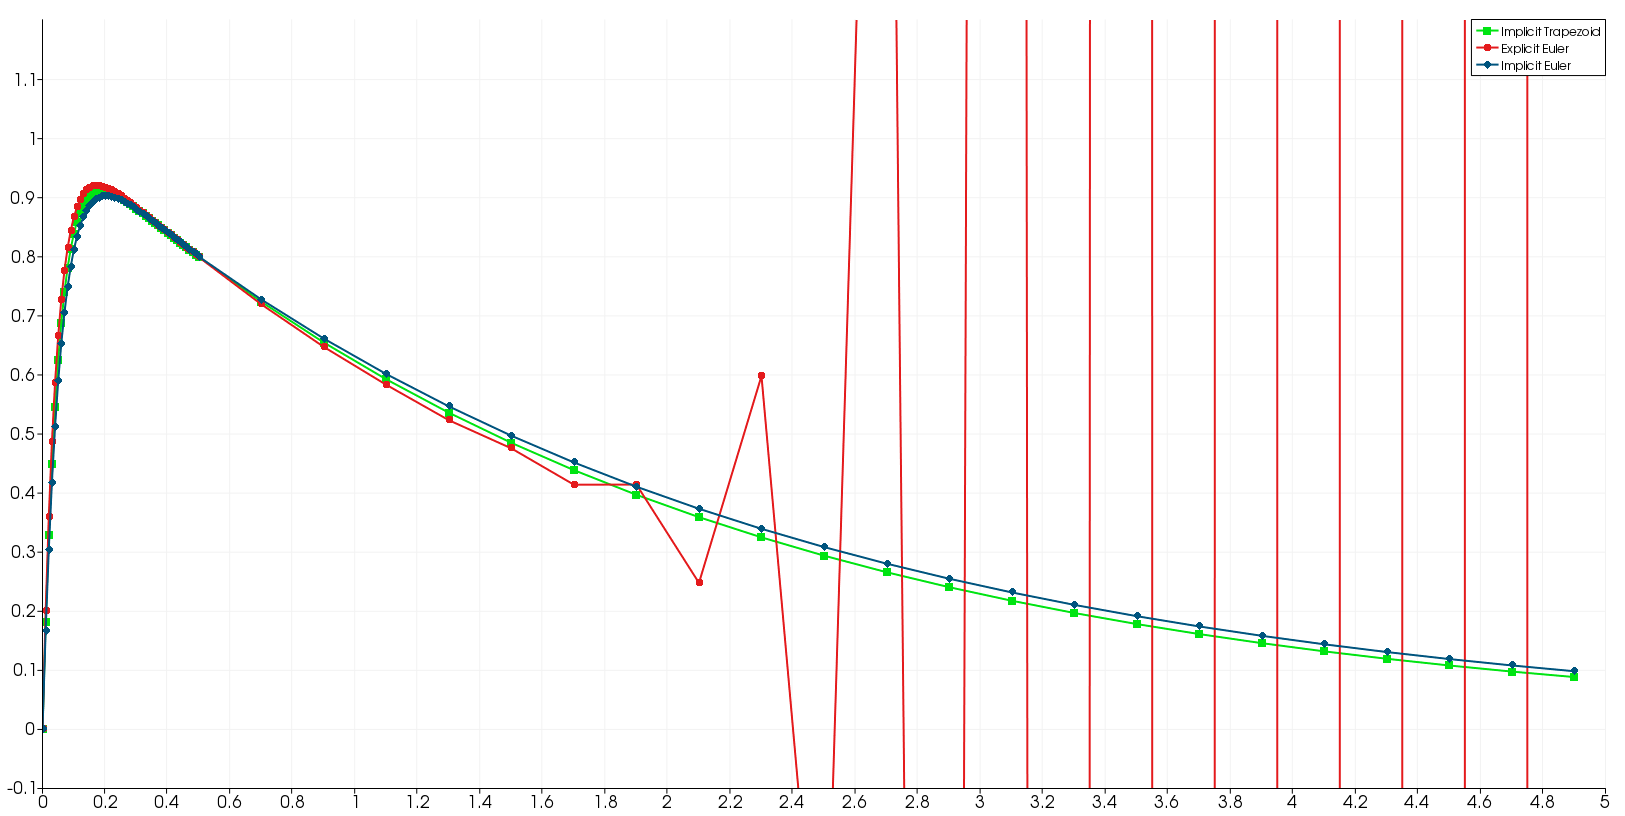
\includegraphics[height=.6\textheight]{fine-coarse.png}}%
	\only<2>{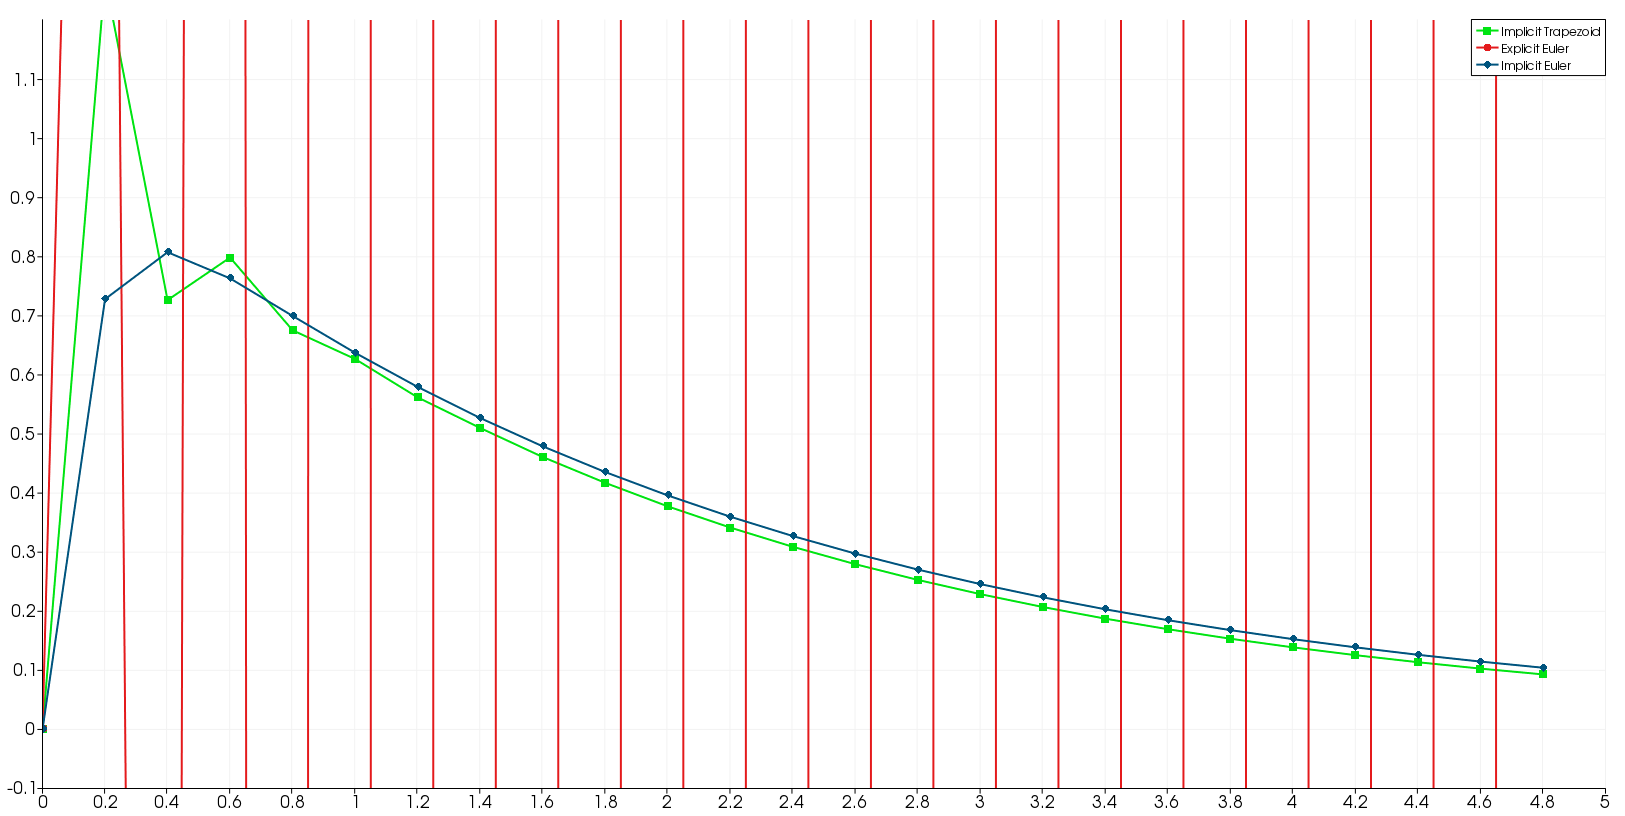
\includegraphics[height=.6\textheight]{coarse.png}}%
	\caption{Решение жесткой задачи разными методами с ограничением шага в
погранслое и без}
	\end{figure}
\end{frame}

\begin{frame}\frametitle{Функция устойчивости методов Рунге-Кутты}
	Для методов Рунге-Кутты функцию устойчивости можно вычислить по формуле
	\[
	r(z) = \frac{\det(\vec E - z\vec A + z\vec 1\vec b^T)}{\det(\vec E - z\vec A)},
	\]
	где $\vec 1$ --- вектор из единиц.
	\pause
	Для случая явного метода, $r(z)$ является многочленом от $z$ степени $s$ (число стадий).
	Но также, $r(z)$ должен с точностью до $O(z^{p+1})$ совпадать с разложением $e^z$ в ряд по $z$ (аппроксимация порядка $p$).
	Если $s = p$, то $r(z)$ есть просто первые $s+1$ членов ряда Тейлора функции $e^z$.
\end{frame}

\begin{frame}\frametitle{Области устойчивости методов Рунге-Кутты 1-4 порядка}
\begin{figure}%
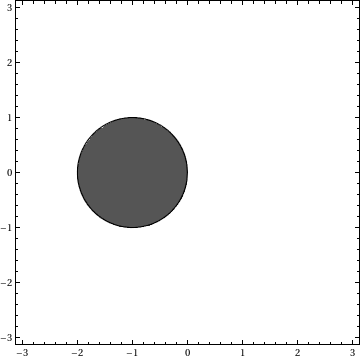
\includegraphics[height=.4\textheight]{rk1.png}%
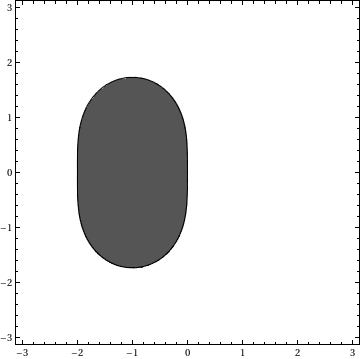
\includegraphics[height=.4\textheight]{rk2.png}%

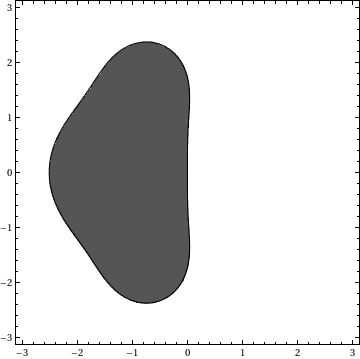
\includegraphics[height=.4\textheight]{rk3.png}%
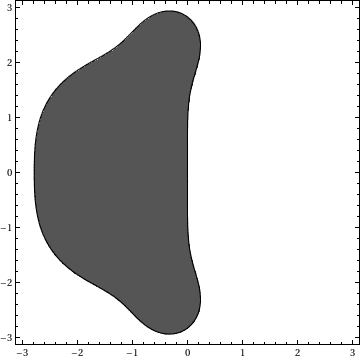
\includegraphics[height=.4\textheight]{rk4.png}%
\end{figure}
\end{frame}

\begin{frame}[plain]
  \begin{center}
  {\Huge Спасибо за внимание!}
  \vspace{8ex}

  Цыбулин Иван

  e-mail: \colorhref{mailto:tsybulin@crec.mipt.ru}{tsybulin@crec.mipt.ru}
  \end{center}
\end{frame}

\end{document}
